\documentclass{beamer}
\usepackage[utf8]{inputenc}

\usetheme{Madrid}
\usecolortheme{default}
\usepackage{amsmath,amssymb,amsfonts,amsthm}
\usepackage{mathtools}
\usepackage{txfonts}
\usepackage{tkz-euclide}
\usepackage{listings}
\usepackage{adjustbox}
\usepackage{array}
\usepackage{gensymb}
\usepackage{tabularx}
\usepackage{gvv}
\usepackage{lmodern}
\usepackage{circuitikz}
\usepackage{tikz}
\lstset{literate={·}{{$\cdot$}}1 {λ}{{$\lambda$}}1 {→}{{$\to$}}1}
\usepackage{graphicx}

\setbeamertemplate{page number in head/foot}[totalframenumber]

\usepackage{tcolorbox}
\tcbuselibrary{minted,breakable,xparse,skins}



\definecolor{bg}{gray}{0.95}
\DeclareTCBListing{mintedbox}{O{}m!O{}}{%
  breakable=true,
  listing engine=minted,
  listing only,
  minted language=#2,
  minted style=default,
  minted options={%
    linenos,
    gobble=0,
    breaklines=true,
    breakafter=,,
    fontsize=\small,
    numbersep=8pt,
    #1},
  boxsep=0pt,
  left skip=0pt,
  right skip=0pt,
  left=25pt,
  right=0pt,
  top=3pt,
  bottom=3pt,
  arc=5pt,
  leftrule=0pt,
  rightrule=0pt,
  bottomrule=2pt,
  toprule=2pt,
  colback=bg,
  colframe=orange!70,
  enhanced,
  overlay={%
    \begin{tcbclipinterior}
    \fill[orange!20!white] (frame.south west) rectangle ([xshift=20pt]frame.north west);
    \end{tcbclipinterior}},
  #3,
}
\lstset{
    language=C,
    basicstyle=\ttfamily\small,
    keywordstyle=\color{blue},
    stringstyle=\color{orange},
    commentstyle=\color{green!60!black},
    numbers=left,
    numberstyle=\tiny\color{gray},
    breaklines=true,
    showstringspaces=false,
}

\title{4.10.15}
\date{September 12, 2025}
\author{Bhargav - EE25BTECH11013}



\begin{document}

\frame{\titlepage}

\begin{frame}{Question}
Show that the lines
\begin{align}
\frac{x-1}{2} = \frac{y-2}{3} = \frac{z-3}{4}
\end{align}
and
\begin{align}
\frac{x-4}{5} = \frac{y-1}{2} = z
\end{align}
intersect. Also, find their point of intersection.
\end{frame}

\begin{frame}{Vector Equations}
The vector equations of the given lines are
\begin{align}
\vec{r}_1 &= \myvec{1\\2\\3} + \lambda \myvec{2\\3\\4}, \\
\vec{r}_2 &= \myvec{4\\1\\0} + \mu \myvec{5\\2\\1}.
\end{align}
At the point of intersection,
\begin{align}
\vec{r}_1 = \vec{r}_2.
\end{align}
\end{frame}

\begin{frame}{Matrix Equation}
Thus,
\begin{align}
\myvec{1\\2\\3} + \lambda \myvec{2\\3\\4} &= \myvec{4\\1\\0} + \mu \myvec{5\\2\\1}.
\end{align}
This can be written as
\begin{align}
\myvec{2 & -5 \\ 3 & -2 \\ 4 & -1}\myvec{\lambda \\ \mu} = \myvec{3 \\ -1 \\ -3}.
\end{align}
\end{frame}

\begin{frame}{Row Reduction}
The corresponding augmented matrix is
\begin{align}
\augvec{2}{1}{2 & -5 &3 \\ 3 & -2 &  -1 \\ 4 & -1 & -3} \xleftrightarrow[R_2 \leftarrow R_2 - \frac{3}{2}R_1]{R_3 \leftarrow R_3 - 2R_1} \augvec{2}{1}{2 & -5 & 3 \\ 0 & 11/2 & -11/2 \\ 0 & 9 & -9}
\end{align}

\begin{align}
\xleftrightarrow[R_3 \leftarrow 11R_3 - 9R_2]{R_2 \leftarrow 2R_2} \augvec{2}{1}{2 & -5 & 3 \\ 0 & 11 & -11 \\ 0 & 0 & 0}
\end{align}
\end{frame}

\begin{frame}{Solution}
From this,
\begin{align}
\myvec{\lambda \\ \mu} = \myvec{-1 \\ -1}.
\end{align}

Substituting into $\vec{r}_1$:

\begin{align}
\vec{r}_1 = \myvec{1\\2\\3} + (-1)\myvec{2\\3\\4} = \myvec{-1\\-1\\-1}.
\end{align}
\end{frame}

\begin{frame}{Intersection Point}
Therefore, the lines intersect at the point
\begin{align}
\myvec{-1\\-1\\-1}
\end{align}
\end{frame}

\begin{frame}{Figure}
\begin{figure}[h!]
    \centering
    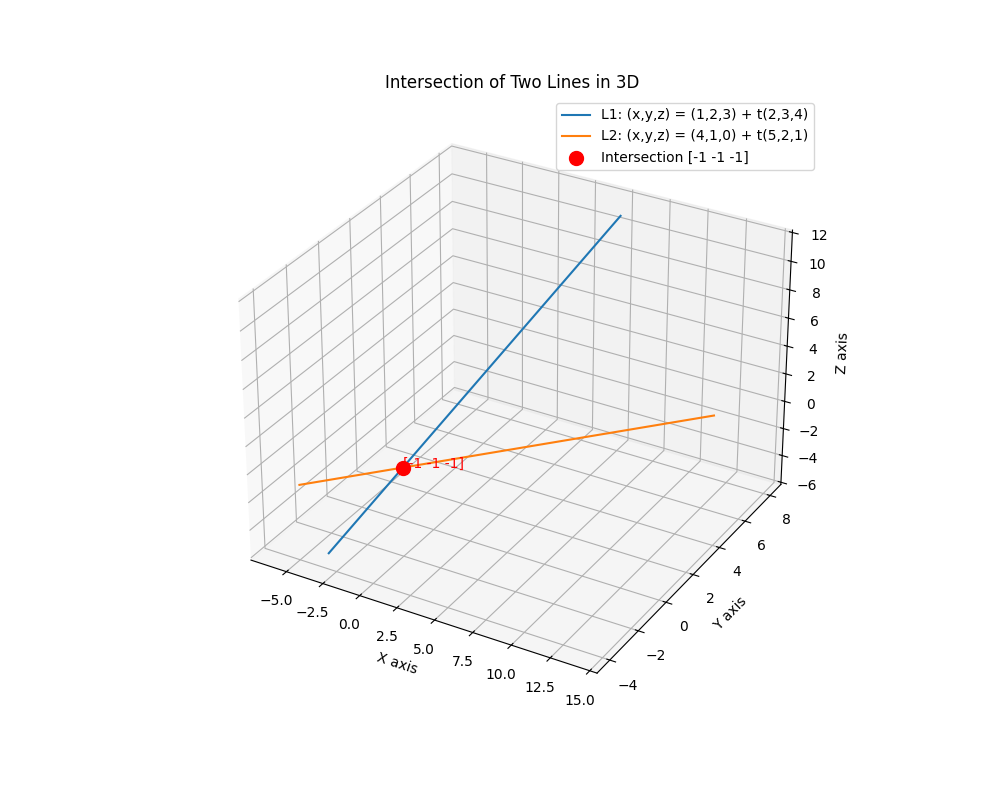
\includegraphics[height=0.5\textheight, keepaspectratio]{figs/Figure_1.png}
\end{figure}
\end{frame}

\begin{frame}[fragile]
    \frametitle{C Code}
    \begin{lstlisting}
#include <stdio.h>
int line_intersection(double p1[3], double d1[3],
                      double p2[3], double d2[3],
                      double intersection[3]) {
    double A[2][2] = {
        { d1[0], -d2[0] },
        { d1[1], -d2[1] }
    };
    double b[2] = { p2[0] - p1[0], p2[1] - p1[1] };

    double det = A[0][0]*A[1][1] - A[0][1]*A[1][0];
    if(det == 0) {
        return -1; // Parallel or skew
    }
    double lam = (b[0]*A[1][1] - b[1]*A[0][1]) / det;
    for(int i = 0; i < 3; i++) {
        intersection[i] = p1[i] + lam*d1[i];
    }
    return 0;
}

    \end{lstlisting}
\end{frame}

\begin{frame}[fragile]
    \frametitle{Python + C Code}
    \begin{lstlisting}
import numpy as np
import matplotlib.pyplot as plt
import ctypes
lib = ctypes.CDLL("./line_intersection.so")
lib.line_intersection.argtypes = [
    np.ctypeslib.ndpointer(ctypes.c_double, ndim=1, flags="C_CONTIGUOUS"),
    np.ctypeslib.ndpointer(ctypes.c_double, ndim=1, flags="C_CONTIGUOUS"),
    np.ctypeslib.ndpointer(ctypes.c_double, ndim=1, flags="C_CONTIGUOUS"),
    np.ctypeslib.ndpointer(ctypes.c_double, ndim=1, flags="C_CONTIGUOUS"),
    np.ctypeslib.ndpointer(ctypes.c_double, ndim=1, flags="C_CONTIGUOUS"),
]
lib.line_intersection.restype = ctypes.c_int
p1, d1 = np.array([1.0, 2.0, 3.0]), np.array([2.0, 3.0, 4.0])
p2, d2 = np.array([4.0, 1.0, 0.0]), np.array([5.0, 2.0, 1.0])


    \end{lstlisting}
\end{frame}

\begin{frame}[fragile]
    \frametitle{Python + C Code}
    \begin{lstlisting}
intersection = np.zeros(3, dtype=np.float64)


status = lib.line_intersection(p1, d1, p2, d2, intersection)
if status != 0:
    print("The lines are parallel or skew; no intersection.")
else:
    print(f"The lines intersect at: {intersection.astype(int)}")


    eq1 = f"L1: (x,y,z) = ({int(p1[0])},{int(p1[1])},{int(p1[2])}) + t({int(d1[0])},{int(d1[1])},{int(d1[2])})"
    eq2 = f"L2: (x,y,z) = ({int(p2[0])},{int(p2[1])},{int(p2[2])}) + t({int(d2[0])},{int(d2[1])},{int(d2[2])})"
    fig = plt.figure(figsize=(10, 8))
    ax = fig.add_subplot(111, projection="3d")
    t = np.linspace(-2, 2, 50)
    \end{lstlisting}
\end{frame}
\begin{frame}[fragile]
    \frametitle{Python + C Code}
    \begin{lstlisting}
    line1_points = p1 + t[:, None] * d1
    line2_points = p2 + t[:, None] * d2
    ax.plot(line1_points[:, 0], line1_points[:, 1], line1_points[:, 2], label=eq1)
    ax.plot(line2_points[:, 0], line2_points[:, 1], line2_points[:, 2], label=eq2)
    ax.scatter(intersection[0], intersection[1], intersection[2],
               color="red", s=100, zorder=5, label=f"Intersection {intersection.astype(int)}")
    ax.text(intersection[0], intersection[1], intersection[2],
            f"{intersection.astype(int)}", color="red", fontsize=10)
    ax.set_xlabel("X axis")
    ax.set_ylabel("Y axis")
    ax.set_zlabel("Z axis")
    ax.set_title("Intersection of Two Lines in 3D")
    ax.legend()
    plt.savefig('/Users/bhargavkrish/Desktop/BackupMatrix/ee25btech11013/matgeo/4.10.15/figs/Figure_1.png')
    plt.show()

    \end{lstlisting}
\end{frame}
\begin{frame}[fragile]
    \frametitle{Python Code}
    \begin{lstlisting}
import numpy as np
import matplotlib.pyplot as plt

p1, d1 = np.array([1, 2, 3]), np.array([2, 3, 4])
p2, d2 = np.array([4, 1, 0]), np.array([5, 2, 1])

A = np.array([d1[:2], -d2[:2]]).T
b = p2[:2] - p1[:2]

try:
    lambda_val, mu_val = np.linalg.solve(A, b)
    intersection_point = p1 + lambda_val * d1
    print(f"The lines intersect at the point: {intersection_point}")

    # Line equations for legend
    eq1 = f"L1: (x,y,z) = ({p1[0]},{p1[1]},{p1[2]}) + t({d1[0]},{d1[1]},{d1[2]})"
    eq2 = f"L2: (x,y,z) = ({p2[0]},{p2[1]},{p2[2]}) + t({d2[0]},{d2[1]},{d2[2]})"

    
    \end{lstlisting}
\end{frame}

\begin{frame}[fragile]
    \frametitle{Python Code}
    \begin{lstlisting}
    fig = plt.figure(figsize=(10, 8))
    ax = fig.add_subplot(111, projection='3d')
    t = np.linspace(-2, 2, 50)
    line1_points = p1 + t[:, np.newaxis] * d1
    line2_points = p2 + t[:, np.newaxis] * d2
    ax.plot(line1_points[:, 0], line1_points[:, 1], line1_points[:, 2], label=eq1)
    ax.plot(line2_points[:, 0], line2_points[:, 1], line2_points[:, 2], label=eq2)
    ax.scatter(intersection_point[0], intersection_point[1], intersection_point[2],
               color='red', s=100, zorder=5, label=f'Intersection {intersection_point}')
    ax.text(intersection_point[0], intersection_point[1], intersection_point[2],
            f'{intersection_point}', color='red', fontsize=10)
    ax.set_xlabel('X axis')
    ax.set_ylabel('Y axis')
    ax.set_zlabel('Z axis')

    \end{lstlisting}
\end{frame}

\begin{frame}[fragile]
    \frametitle{Python Code}
    \begin{lstlisting}
    ax.set_title('Intersection of Two Lines in 3D')
    ax.legend()
    plt.savefig('/Users/bhargavkrish/Desktop/BackupMatrix/ee25btech11013/matgeo/4.10.15/figs/Figure_1.png')
    plt.show()

except np.linalg.LinAlgError:
    print("The lines are parallel or skew; they do not intersect.")

    \end{lstlisting}
\end{frame}
    
\end{document}
